\documentclass{article}
\usepackage[utf8]{inputenc}
\usepackage{subfig}

%References
\usepackage{natbib}
%IMPORTANT use https://www.citationmachine.net/ if you need to generate references!
% \citep{reference} creates Harvard Style references throughout

%Colors
\usepackage{xcolor}

\usepackage[protrusion=true,expansion]{microtype}

%Code Markup
\usepackage[outputdir=cache]{minted}
%Syntax Highlighting Style
\definecolor{bggray}{RGB}{40,40,40}
%Macro to make a Syntax Highlighter For Java files 
%Use \javacode{filename.java} to insert a Java File W/ Syntax Highlighting file into the PDF
\newmintedfile[javacode]{java}{
	style=fruity,
	bgcolor=bggray,
	linenos,
	breaklines,
	tabsize=2,
	obeytabs
}

\newmintedfile[bashoutput]{txt}{
	style=fruity,
	bgcolor=lightgray,
	breaklines,
	tabsize=2,
	obeytabs
}

%Page Margins and stuff
\usepackage{geometry}
 \geometry{
 a4paper,
 total={170mm,257mm},
 left=20mm,
 }

%Pictures
\usepackage{graphicx}
\graphicspath{ {./images/} }

%Move the title position
\usepackage{titling}

\setlength{\droptitle}{-8.5em} %Up, near the top but not too high

\title{Assignment 3 - Software Engineering 3}
\author{Daniel Hannon (19484286)}
\date{Novemeber 2021}

\begin{document}
	\maketitle
	%Sets to Harvard Style and links the references file
	\section{Outline}
	\subsection{Setup}
	In order to commece this assignment, I had to setup hibernate on my machine. I downloaded the archetype from the notes and it kept spitting out ``does not opens java.lang to unnamed module'' no matter what I did, it included rolling back to java 8 and several other fixes.After 5 hours I came up with a workaround In order to circumvent this I just used the simple-webapp archetype that was used in the previous two assignments.  In order to verify that it worked, I wrote a simple script to connect to the database via hibernate and create an entry. It luckily worked first time.
	\begin{figure}[h!]
		\centering
		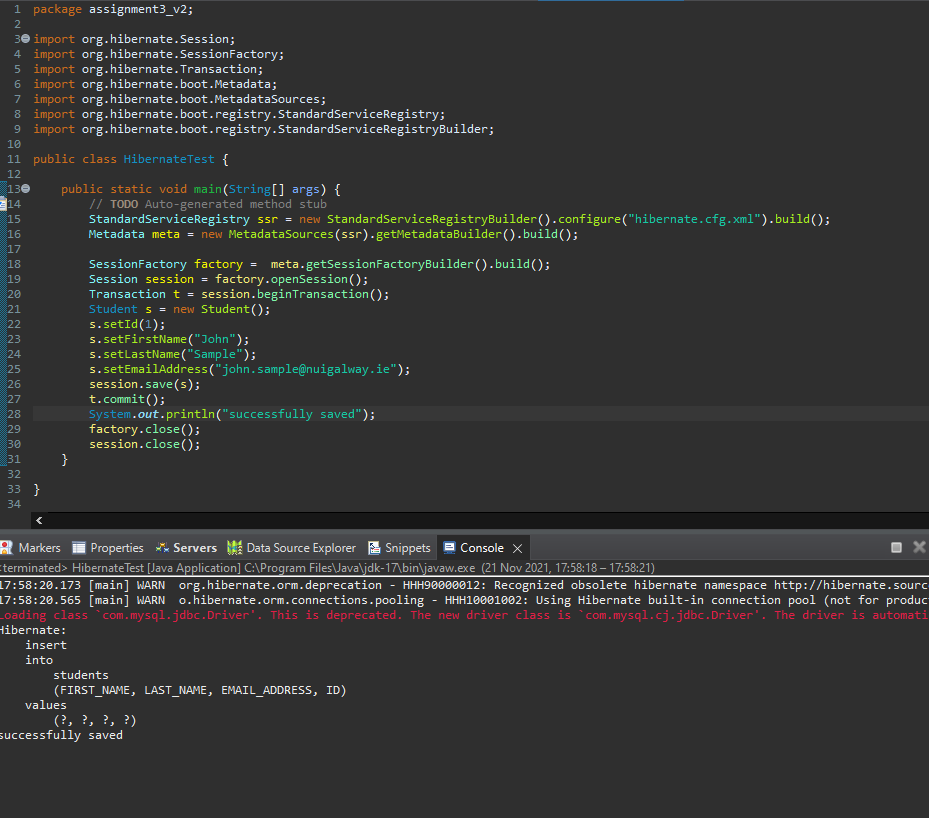
\includegraphics[width=0.7\textwidth]{1.png}
	\end{figure}
	\section{create}
With this I had to create the create functionality. I took a lot of inspiration from the update servlet I wrote for the last assignment and wrote a Class to handle creating a hashmap of the query string as it made parsing much more scalable. then beyond this it was very straightforward. When it creates the the entry it shows it in the view students so you can get your email and idno as they are not decided by the user.
	\begin{figure}[h!]
		\centering
		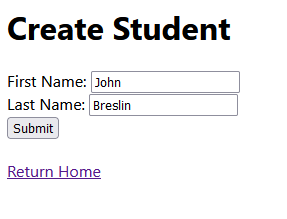
\includegraphics[width=0.7\textwidth]{2.png}
	\end{figure}
	\\
	\begin{figure}[h!]
		\centering
		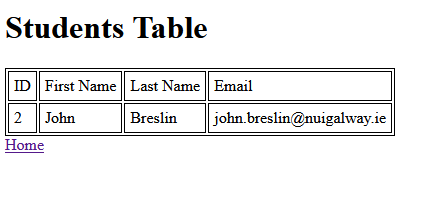
\includegraphics[width=0.7\textwidth]{3.png}
	\end{figure}
	\\
	Additionally it handles with duplicate emails in the manner as requested\\
	\begin{figure}[h!]
		\centering
		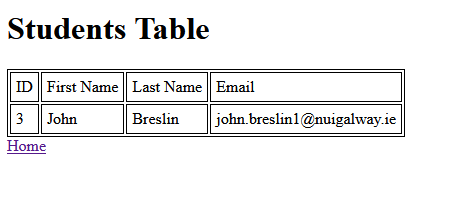
\includegraphics[width=0.7\textwidth]{4.png}
	\end{figure}
	\newpage
	\section{read}
		I wrote the Read servlet to handle either the id parameter or none, if none are passed I show everyhting otherwise I show the record associated with the ID. this is used to show the newly created records using create.
		\begin{figure}[h!]
			\centering
			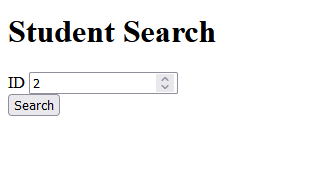
\includegraphics[width=0.7\textwidth]{5.png}
		\end{figure}
		\newpage
		
	\section{Delete}
		Delete Functionality only works on the id parameter
		
		\begin{figure}[h!]
			\centering
			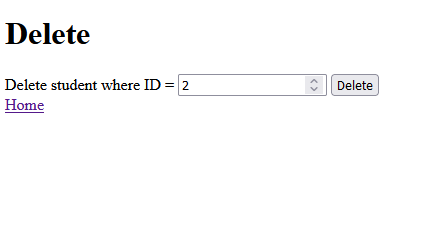
\includegraphics[width=0.7\textwidth]{6.png}
		\end{figure}
		
		\begin{figure}[h!]
			\centering
			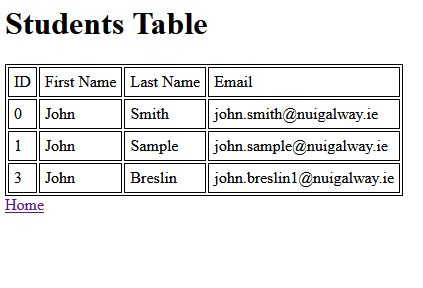
\includegraphics[width=0.7\textwidth]{7.png}
		\end{figure}
	\section{update}
	With Update I  took a similar approach as I did for the previous assignment. with the batch email update function I check for duplicates on every email when I change them as there's a chance you're turning back to nuigalway.ie and then there might be a dupe.
	
		\begin{figure}[h!]
			\centering
			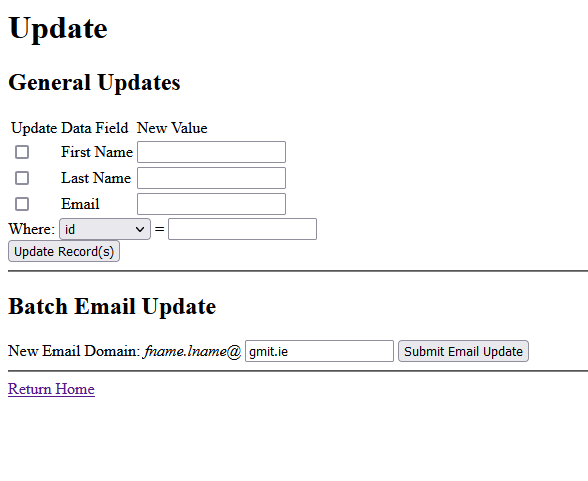
\includegraphics[width=0.7\textwidth]{8.png}
		\end{figure}
		
		\begin{figure}[h!]
			\centering
			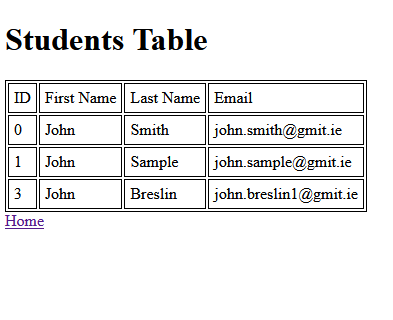
\includegraphics[width=0.7\textwidth]{9.png}
		\end{figure}
		
		\begin{figure}[h!]
			\centering
			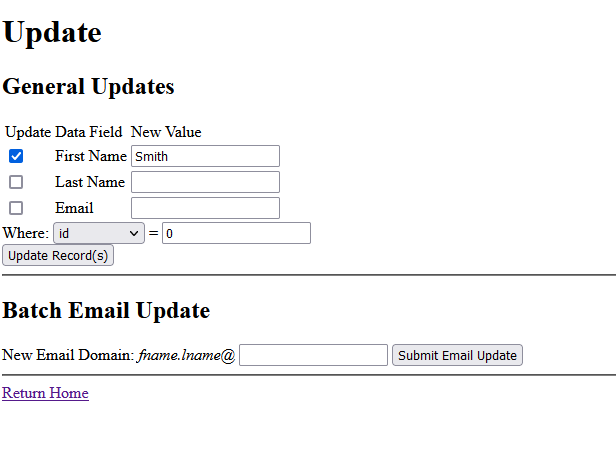
\includegraphics[width=0.7\textwidth]{10.png}
		\end{figure}
		
		\begin{figure}[h!]
			\centering
			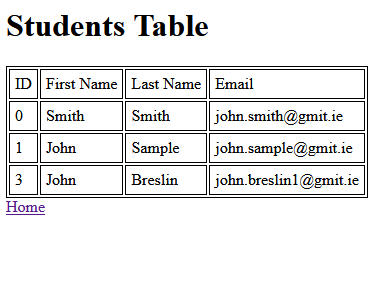
\includegraphics[width=0.7\textwidth]{11.png}
		\end{figure}
	\section{Extras}
	I allow you to perform batch updates on several fields with update and you do not need to update every parameter
	Error page redirect
	If the operation is successful, you can immediately see it's result
	\bibliographystyle{agsm}
	\bibliography{references}
\end{document}